\documentclass{uebblatt}

\newcommand{\cont}{\mathrm{cont}}
\newcommand{\http}{http:/\kern-.2em/\kern-0.03em}

\begin{document}

\maketitle{14}{}

\vfill

\begin{aufgabe}{0}{Rationale Binomialkoeffizienten}
\small
Für rationale Zahlen~$x$ und natürliche Zahlen~$k$ setzen wir~$\binom{x}{k}
\defeq x (x-1) \cdots (x-k+1) / k! \in \QQ$. Solche Binomialkoeffizienten
kommen in Taylor-Entwicklungen vieler wichtiger Funktionen vor.
\begin{enumerate}
\item Zeige: Genau dann kommt im gekürzten Nenner einer rationalen Zahl~$a/b$
nicht der Primfaktor~$p$ vor, wenn es eine~$p$-adische Ganzzahl~$u$ mit~$bu = a$ gibt.
\item Verwende die Dichtheit von~$\ZZ$ in~$\ZZ_p$ und die Stetigkeit von
Polynomen über~$\ZZ_p$, um zu folgern: Im gekürzten Nenner eines rationalen
Binomialkoeffizienten~$\binom{x}{k}$ können nur solche Primfaktoren vorkommen, die auch
im gekürzten Nenner von~$x$ vorkommen.
\end{enumerate}
\end{aufgabe}

\centering
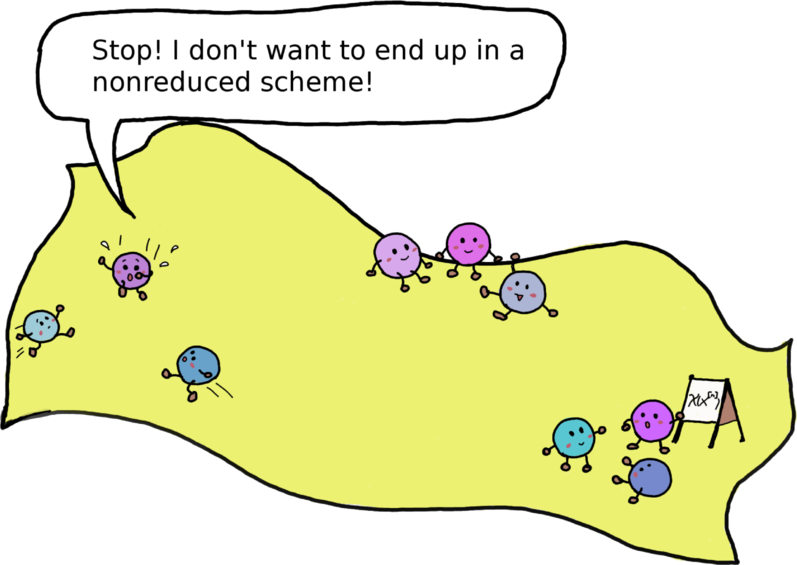
\includegraphics{images/hilbert-scheme-of-points}

\end{document}
